\subsection{UC-16}
\label{subsec:UC-16}

\begin{figure}[H]
    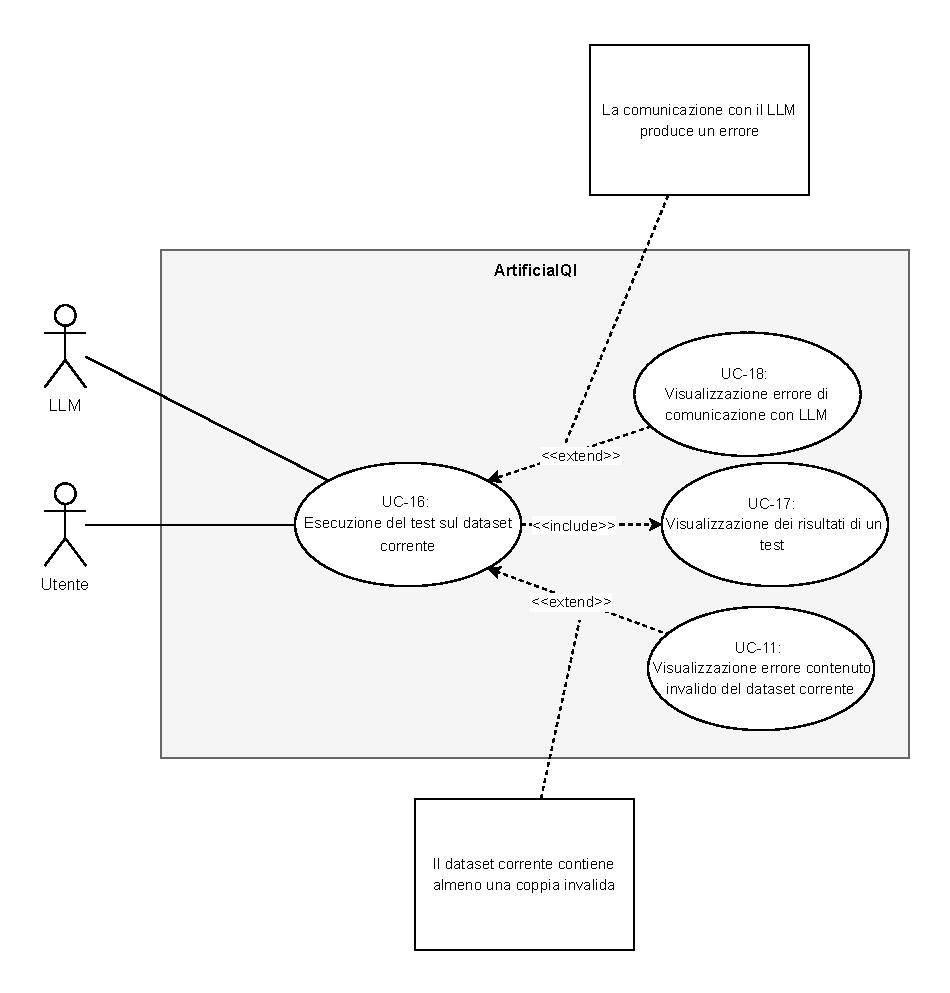
\includegraphics[scale=0.8]{Sezioni/UseCase/Immagini/UC-16.pdf}
    \caption{Diagramma UC-16.}
\end{figure}

\begin{usecase}{UC-16}{Esecuzione del test sul dataset caricato}

    \req{\hyperref[item:RU-5]{RU-5}} 

    \pre{
        \item Il sistema è attivo e funzionante
        \item Il dataset caricato non è vuoto
    }

    \post{
        \item L'utente conosce l'esito del test
    }
    
    \actor{Utente}

    \subactors{LLM}

    \trigger{L'utente deve testare il LLM usando il dataset caricato}
    
    \inc{\hyperref[subsec:UC-17]{UC-17}}

    \base{}

    \scenario{
        \item L'utente richiede l'esecuzione del test
        \item Per ogni coppia del dataset caricato si ottiene la risposta prodotta dal LLM sotto test
        \item Per ogni coppia del dataset caricato si calcola il grado di somiglianza tra la risposta prodotta dal LLM sotto test rispetto alla risposta attesa
        \item \texttt{<<include:UC-17>>}
    }

    \subscenario{
        \item[1.1] \textbf{Il dataset caricato contiene almeno una coppia invalida}
        \begin{itemize}
            \item[a.] hyperref[subsec:UC-11]{UC-11}
        \end{itemize}
        \item[2.1] \textbf{La comunicazione con LLM produce un errore}
        \begin{itemize}
        \item[a.] \hyperref[subsec:UC-18]{UC-18}
        \end{itemize}
    }
\end{usecase}